% Options for packages loaded elsewhere
% Options for packages loaded elsewhere
\PassOptionsToPackage{unicode}{hyperref}
\PassOptionsToPackage{hyphens}{url}
\PassOptionsToPackage{dvipsnames,svgnames,x11names}{xcolor}
%
\documentclass[
  twoside,
  symmetric]{tufte-book}
\usepackage{xcolor}
\usepackage{amsmath,amssymb}
\setcounter{secnumdepth}{-\maxdimen} % remove section numbering
\usepackage{iftex}
\ifPDFTeX
  \usepackage[T1]{fontenc}
  \usepackage[utf8]{inputenc}
  \usepackage{textcomp} % provide euro and other symbols
\else % if luatex or xetex
  \usepackage{unicode-math} % this also loads fontspec
  \defaultfontfeatures{Scale=MatchLowercase}
  \defaultfontfeatures[\rmfamily]{Ligatures=TeX,Scale=1}
\fi
\usepackage{lmodern}
\ifPDFTeX\else
  % xetex/luatex font selection
\fi
% Use upquote if available, for straight quotes in verbatim environments
\IfFileExists{upquote.sty}{\usepackage{upquote}}{}
\IfFileExists{microtype.sty}{% use microtype if available
  \usepackage[]{microtype}
  \UseMicrotypeSet[protrusion]{basicmath} % disable protrusion for tt fonts
}{}
\makeatletter
\@ifundefined{KOMAClassName}{% if non-KOMA class
  \IfFileExists{parskip.sty}{%
    \usepackage{parskip}
  }{% else
    \setlength{\parindent}{0pt}
    \setlength{\parskip}{6pt plus 2pt minus 1pt}}
}{% if KOMA class
  \KOMAoptions{parskip=half}}
\makeatother
% Make \paragraph and \subparagraph free-standing
\makeatletter
\ifx\paragraph\undefined\else
  \let\oldparagraph\paragraph
  \renewcommand{\paragraph}{
    \@ifstar
      \xxxParagraphStar
      \xxxParagraphNoStar
  }
  \newcommand{\xxxParagraphStar}[1]{\oldparagraph*{#1}\mbox{}}
  \newcommand{\xxxParagraphNoStar}[1]{\oldparagraph{#1}\mbox{}}
\fi
\ifx\subparagraph\undefined\else
  \let\oldsubparagraph\subparagraph
  \renewcommand{\subparagraph}{
    \@ifstar
      \xxxSubParagraphStar
      \xxxSubParagraphNoStar
  }
  \newcommand{\xxxSubParagraphStar}[1]{\oldsubparagraph*{#1}\mbox{}}
  \newcommand{\xxxSubParagraphNoStar}[1]{\oldsubparagraph{#1}\mbox{}}
\fi
\makeatother


\usepackage{longtable,booktabs,array}
\usepackage{calc} % for calculating minipage widths
% Correct order of tables after \paragraph or \subparagraph
\usepackage{etoolbox}
\makeatletter
\patchcmd\longtable{\par}{\if@noskipsec\mbox{}\fi\par}{}{}
\makeatother
% Allow footnotes in longtable head/foot
\IfFileExists{footnotehyper.sty}{\usepackage{footnotehyper}}{\usepackage{footnote}}
\makesavenoteenv{longtable}
\usepackage{graphicx}
\makeatletter
\newsavebox\pandoc@box
\newcommand*\pandocbounded[1]{% scales image to fit in text height/width
  \sbox\pandoc@box{#1}%
  \Gscale@div\@tempa{\textheight}{\dimexpr\ht\pandoc@box+\dp\pandoc@box\relax}%
  \Gscale@div\@tempb{\linewidth}{\wd\pandoc@box}%
  \ifdim\@tempb\p@<\@tempa\p@\let\@tempa\@tempb\fi% select the smaller of both
  \ifdim\@tempa\p@<\p@\scalebox{\@tempa}{\usebox\pandoc@box}%
  \else\usebox{\pandoc@box}%
  \fi%
}
% Set default figure placement to htbp
\def\fps@figure{htbp}
\makeatother





\setlength{\emergencystretch}{3em} % prevent overfull lines

\providecommand{\tightlist}{%
  \setlength{\itemsep}{0pt}\setlength{\parskip}{0pt}}



 
\usepackage[]{natbib}
\bibliographystyle{plainnat}


\usepackage{lipsum}
\usepackage{graphicx}
\graphicspath{{style-guide/graphics/}}
% Redefine commands to avoid conflicts
\providecommand{\TL}{Tufte-\LaTeX}
\makeatletter
\@ifpackageloaded{caption}{}{\usepackage{caption}}
\AtBeginDocument{%
\ifdefined\contentsname
  \renewcommand*\contentsname{Table of contents}
\else
  \newcommand\contentsname{Table of contents}
\fi
\ifdefined\listfigurename
  \renewcommand*\listfigurename{List of Figures}
\else
  \newcommand\listfigurename{List of Figures}
\fi
\ifdefined\listtablename
  \renewcommand*\listtablename{List of Tables}
\else
  \newcommand\listtablename{List of Tables}
\fi
\ifdefined\figurename
  \renewcommand*\figurename{Figure}
\else
  \newcommand\figurename{Figure}
\fi
\ifdefined\tablename
  \renewcommand*\tablename{Table}
\else
  \newcommand\tablename{Table}
\fi
}
\@ifpackageloaded{float}{}{\usepackage{float}}
\floatstyle{ruled}
\@ifundefined{c@chapter}{\newfloat{codelisting}{h}{lop}}{\newfloat{codelisting}{h}{lop}[chapter]}
\floatname{codelisting}{Listing}
\newcommand*\listoflistings{\listof{codelisting}{List of Listings}}
\makeatother
\makeatletter
\makeatother
\makeatletter
\@ifpackageloaded{caption}{}{\usepackage{caption}}
\@ifpackageloaded{subcaption}{}{\usepackage{subcaption}}
\makeatother
\makeatletter
\@ifpackageloaded{sidenotes}{}{\usepackage{sidenotes}}
\@ifpackageloaded{marginnote}{}{\usepackage{marginnote}}
\makeatother
\usepackage{bookmark}
\IfFileExists{xurl.sty}{\usepackage{xurl}}{} % add URL line breaks if available
\urlstyle{same}
\hypersetup{
  pdftitle={A Tufte-Style Book},
  pdfauthor={The Tufte-LaTeX Developers},
  colorlinks=true,
  linkcolor={blue},
  filecolor={Maroon},
  citecolor={Blue},
  urlcolor={Blue},
  pdfcreator={LaTeX via pandoc}}


\title{A Tufte-Style Book}
\usepackage{etoolbox}
\makeatletter
\providecommand{\subtitle}[1]{% add subtitle to \maketitle
  \apptocmd{\@title}{\par {\large #1 \par}}{}{}
}
\makeatother
\subtitle{Thanks to Edward R. Tufte for his inspiration}
\author{The Tufte-LaTeX Developers}
\date{2025-05-24}
\begin{document}
\frontmatter
\maketitle


\mainmatter
\chapter*{Introduction}\label{introduction}
\addcontentsline{toc}{chapter}{Introduction}

This sample book discusses the design of Edward Tufte's
books\citep{Tufte2001, Tufte1990, Tufte1997, Tufte2006} and the use of
the \texttt{tufte-book} and \texttt{tufte-handout} document classes.

\chapter{The Design of Tufte's Books}\label{the-design-of-tuftes-books}

The pages of a book are usually divided into three major sections: the
front matter (also called preliminary matter or prelim), the main matter
(the core text of the book), and the back matter (or end matter).

The front matter of a book refers to all of the material that comes
before the main text. The following table shows a list of material that
appears in the front matter of \emph{VDQI}, \emph{EI}, \emph{VE}, and
\emph{BE} along with its page number.

\begin{longtable}[]{@{}lcccc@{}}
\caption{Front matter pages across Tufte's books}\tabularnewline
\toprule\noalign{}
Page content & VDQI & EI & VE & BE \\
\midrule\noalign{}
\endfirsthead
\toprule\noalign{}
Page content & VDQI & EI & VE & BE \\
\midrule\noalign{}
\endhead
\bottomrule\noalign{}
\endlastfoot
Blank half title page & (1) & (1) & (1) & (1) \\
Frontispiece & (2) & (2) & (2) & (2) \\
Full title page & (3) & (3) & (3) & (3) \\
Copyright page & (4) & (4) & (4) & (4) \\
Contents & (5) & (5) & (5) & (5) \\
Dedication & (6) & (7) & (7) & 7 \\
Introduction & (7) & (9) & (9) & 9 \\
\end{longtable}

\section{Typefaces}\label{typefaces}

Tufte's books primarily use two typefaces: Bembo and Gill Sans. Bembo is
used for the headings and body text, while Gill Sans is used for the
title page and opening epigraphs.

Since neither Bembo nor Gill Sans are available in default LaTeX
installations, the Tufte-LaTeX document classes default to using
Palatino and Helvetica, respectively.

\section{Sidenotes}\label{sidenotes}

One of the most prominent and distinctive features of this style is the
extensive use of sidenotes.\footnote{This is a sidenote that was entered
  using the footnote syntax.} There is a wide margin to provide ample
room for sidenotes and small figures.

\section{Figures and Tables}\label{figures-and-tables}

Images and graphics play an integral role in Tufte's work. In addition
to the standard figure and table environments, this style provides
special figure and table environments for full-width floats.

\begin{figure}[H]

{\centering 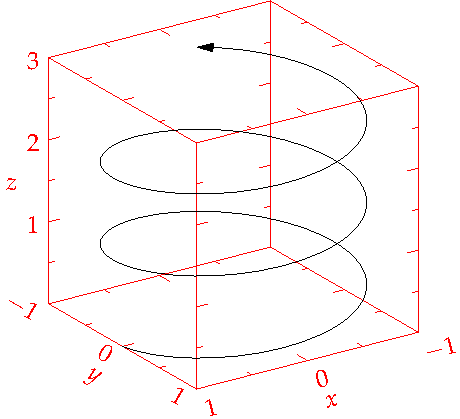
\includegraphics[width=0.5\linewidth,height=\textheight,keepaspectratio]{style-guide/graphics/helix.pdf}

}

\caption{This is a margin figure. The helix is defined by
\(x = \cos(2\pi z)\), \(y = \sin(2\pi z)\), and \(z = [0, 2.7]\).}

\end{figure}%

\begin{figure*}[H]

{\centering \pandocbounded{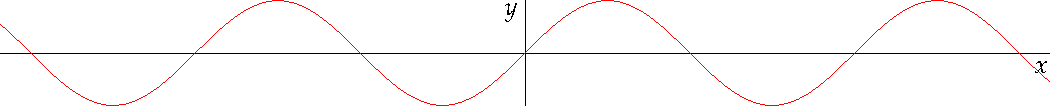
\includegraphics[keepaspectratio]{style-guide/graphics/sine.pdf}}

}

\caption{This graph shows \(y = \sin x\) from about \(x = [-10, 10]\).
\emph{Notice that this figure takes up the full page width.}}

\end{figure*}%

\begin{figure}[H]

{\centering 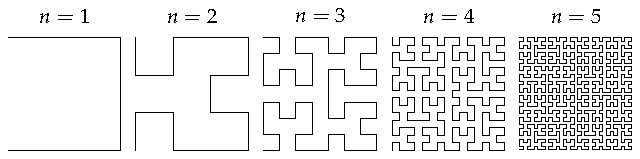
\includegraphics[width=0.7\linewidth,height=\textheight,keepaspectratio]{style-guide/graphics/hilbertcurves.pdf}

}

\caption{Hilbert curves of various degrees \(n\). \emph{Notice that this
figure only takes up the main textblock width.}}

\end{figure}%

\begin{longtable}[]{@{}ll@{}}
\caption{Dimensions of the various margins used in the Tufte-handout
class}\tabularnewline
\toprule\noalign{}
Margin & Length \\
\midrule\noalign{}
\endfirsthead
\toprule\noalign{}
Margin & Length \\
\midrule\noalign{}
\endhead
\bottomrule\noalign{}
\endlastfoot
Paper width & 8½ inches \\
Paper height & 11 inches \\
Textblock width & 6½ inches \\
Textblock/sidenote gutter & ⅜ inches \\
Sidenote width & 2 inches \\
\end{longtable}

\chapter{On the Use of the tufte-book Document
Class}\label{on-the-use-of-the-tufte-book-document-class}

The Tufte-LaTeX document classes define a style similar to the style
Edward Tufte uses in his books and handouts. Tufte's style is known for
its extensive use of sidenotes, tight integration of graphics with text,
and well-set typography.

\section{Page Layout}\label{page-layout}

This style provides \textbf{A}- and \textbf{B}-heads (that is,
\texttt{\textbackslash{}section} and
\texttt{\textbackslash{}subsection}), demonstrated above.

If you need more than two levels of section headings, you'll have to
define them yourself at the moment; there are no pre-defined styles for
anything below a \texttt{\textbackslash{}subsection}.

\section{Typography}\label{typography}

When setting strings of ALL CAPS or small caps, the letterspacing---that
is, the spacing between the letters---should be increased
slightly\citep{Bringhurst2005}.

\section{Document Class Options}\label{document-class-options}

The \texttt{tufte-book} class is based on the LaTeX \texttt{book}
document class. Therefore, you can pass any of the typical book options.
There are a few options that are specific to the \texttt{tufte-book}
document class, however.

The \texttt{a4paper} option will set the paper size to A4 instead of the
default US letter size.

The \texttt{twoside} option will modify the running heads so that the
page number is printed on the outside edge.

The \texttt{symmetric} option typesets the sidenotes on the outside edge
of the page. This is how books are traditionally printed, but is
contrary to Tufte's book design which sets the sidenotes on the right
side of the page.

\chapter*{References}\label{references}
\addcontentsline{toc}{chapter}{References}

\renewcommand{\bibsection}{}
\bibliography{style-guide/sample-handout.bib}


\backmatter



\end{document}
